\section{Magnitude Functions} \label{Sec: Magnitude Functions}

In practice, galaxy luminosity is calculated from the \textit{flux} measurement. Flux is measured in $W/m^2$ (or $J/s/m^2$ in base SI units), the energy received per second over a given area. However, observing telescopes like the \textit{Spitzer Space Telescope} measure \textit{flux density} through filters that only capture light in specific frequency bands and are measured in \textit{Janksys}. \gls{zfourge} measures flux density in $\mu Jy$ which is then converted into \textit{apparent magnitude} using \cref{EQ: Apparent Magnitude}: 

\begin{equation}
    m_{x} = -5 \log_{100} \left(\frac{F_{x}}{F_{x,0}}\right)
    \label{EQ: Apparent Magnitude}
\end{equation}
\myequations{Apparent Magnitude}

where $m_x$ is the apparent magnitude in filter $x$; $F_x$ is the flux density in filter $x$; and $F_{x,0}$ is the reference flux (zero-point) in filter $x$. \gls{zfourge} measures flux density in many bands, but we first test our method of calculating magnitude functions in the $K_{s}$ band. This requires a different method of calculating the \gls{lf} as a few extra steps are required to meet the completeness of the survey. Firstly, the magnitude limit in the $K_{s}$ band is $K_{s,lim} = 25.9\ AB$. Apparent magnitudes can be converted to \textit{AB magnitudes} with \cref{EQ: AB Magnitude}:

\begin{equation}
    M_{AB} = 25 - 2.5 \log_{10}(m_x)
    \label{EQ: AB Magnitude}
\end{equation}
\myequations{AB Magnitude}

Finally, AB magnitude is converted into \textit{absolute magnitude}, which is the apparent magnitude a celestial object would have if it were located at a distance of 10 parsecs and is given by \cref{EQ: Absolute Magnitude}:

\begin{equation}
    M_{abs} = M_{AB} - 5 \log_{10} \left(\frac{d}{10}\right)
    \label{EQ: Absolute Magnitude}
\end{equation}
\myequations{Absolute Magnitude}

Where $d$ is distance measured in units of parsecs. We calculate the distance to each galaxy using the \texttt{Astropy} python package \citep{astropy_collaboration_astropy_2022}. Specifically, the following Python code is used:

\vspace{1.5cm}
\begin{python}    
    # Cosmology
    cosmo = FlatLambdaCDM(H0=70, Om0=0.3)
    
    # Luminosity distance
    d_c = cosmo.comoving_distance(z) * 10 ** 6 # Mpc -> pc
    d_L = cosmo.luminosity_distance(z) * 10 ** 6 # Mpc -> pc
\end{python}

Where $z$ is each galaxy's photometric redshift, or spectroscopic redshift if available. The \texttt{luminosity\_distance} $(d_L)$ and \texttt{comoving\_distance} $(d_C)$ measure two separate distances. $d_C$ does not factor the expansion of the universe and is especially useful in \gls{lf} calculations because it keeps the volume of observed space consistent (\cref{EQ: Vmax}) across all cosmic time. Otherwise, $d_L$ will include the universe's expansion, which inherently disperses galaxies and leads to incorrect number density calculations (\cref{EQ: Number Density}). However, $d_L$ is still useful because it can be used as a luminosity completeness limit, although we define our luminosity completeness limit as simply the turnover point in the luminosity function or number density counts. \Cref{Fig: Magnitude Distribution} shows the absolute magnitude calculated with both $d_C$ and $d_L$. The apparent magnitude limit in the $K_{s}$ band ($K_{s,lim} = 25.9\ AB$) is applied and removes galaxies with AB magnitudes fainter (more positive; above) than $25.9\ AB$.

\begin{figure}[t!]
    \centering
    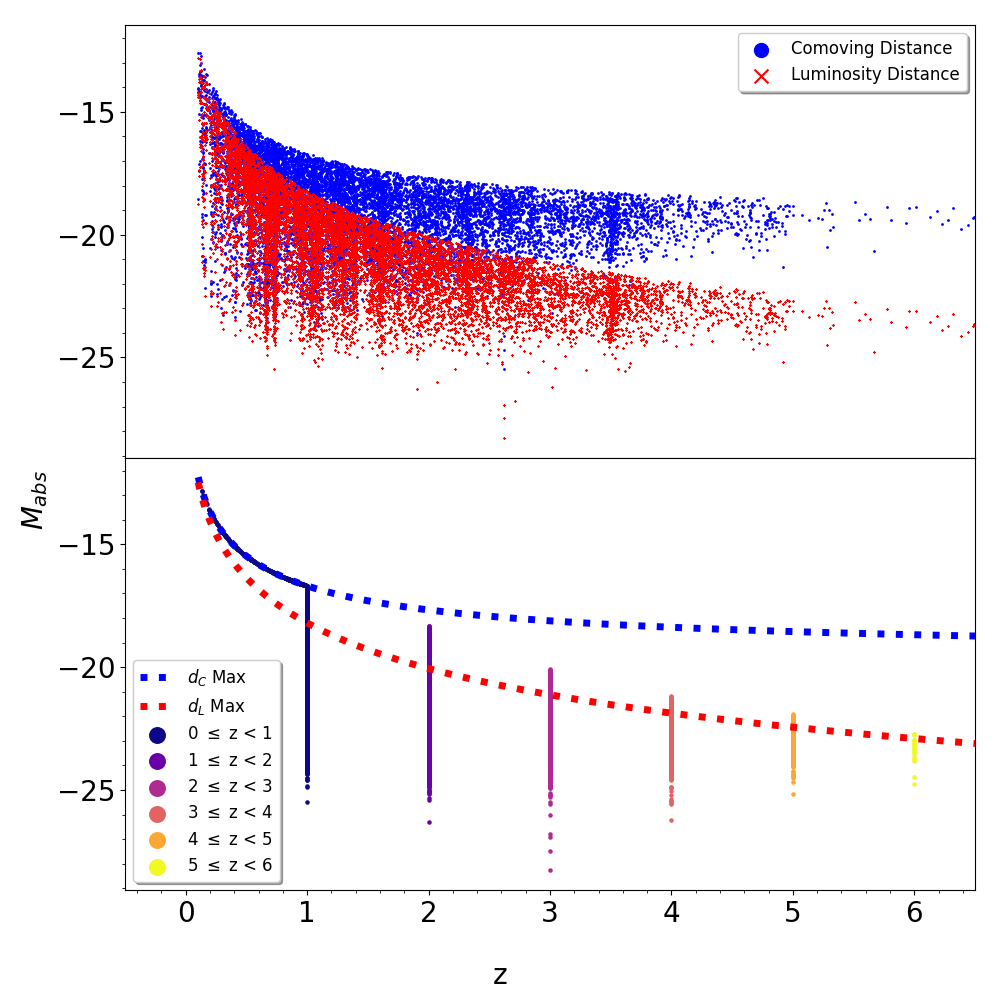
\includegraphics[width=\textwidth]{Figures/Magnitude Distribution.png}
    \caption{ZFOURGE CDFS $K_s$ band magnitude distribution as a function of redshift. Galaxies are masked with $K_{s,lim}$. \textit{Top:} magnitudes calculated with $d_C$ and $d_L$ using \cite{astropy_collaboration_astropy_2022}. \textit{Bottom:} the maximum distance of each galaxy according to the redshift bin it resides in using equation \ref{EQ: Magnitude Dmax}.}
    \label{Fig: Magnitude Distribution}
\end{figure}

$d_{max}$ refers to the distance an object would appear at given it has the same magnitude but if the flux density was at the detectable threshold of the survey. Decreasing flux but keeping luminosity constant means that distance must be the variable changing (increasing). Rearranging \cref{EQ: Absolute Magnitude}, distance can be swapped for $d_{max}$ if $M_{AB}$ is replaced with the magnitude limit. In this case the magnitude limit is $K_{s,lim} = 25.9$ and $d_{max}$ is given by \cref{EQ: Magnitude Dmax}:

\begin{equation}
    d_{max}\ [pc] = 10 \times 10^{\textstyle{\left(\frac{K_{s,lim} - M_{abs}}{5}\right)}}
    \label{EQ: Magnitude Dmax}
\end{equation}
\myequations{Magnitude $d_{max}$}

\begin{figure}[t!]
    \centering
    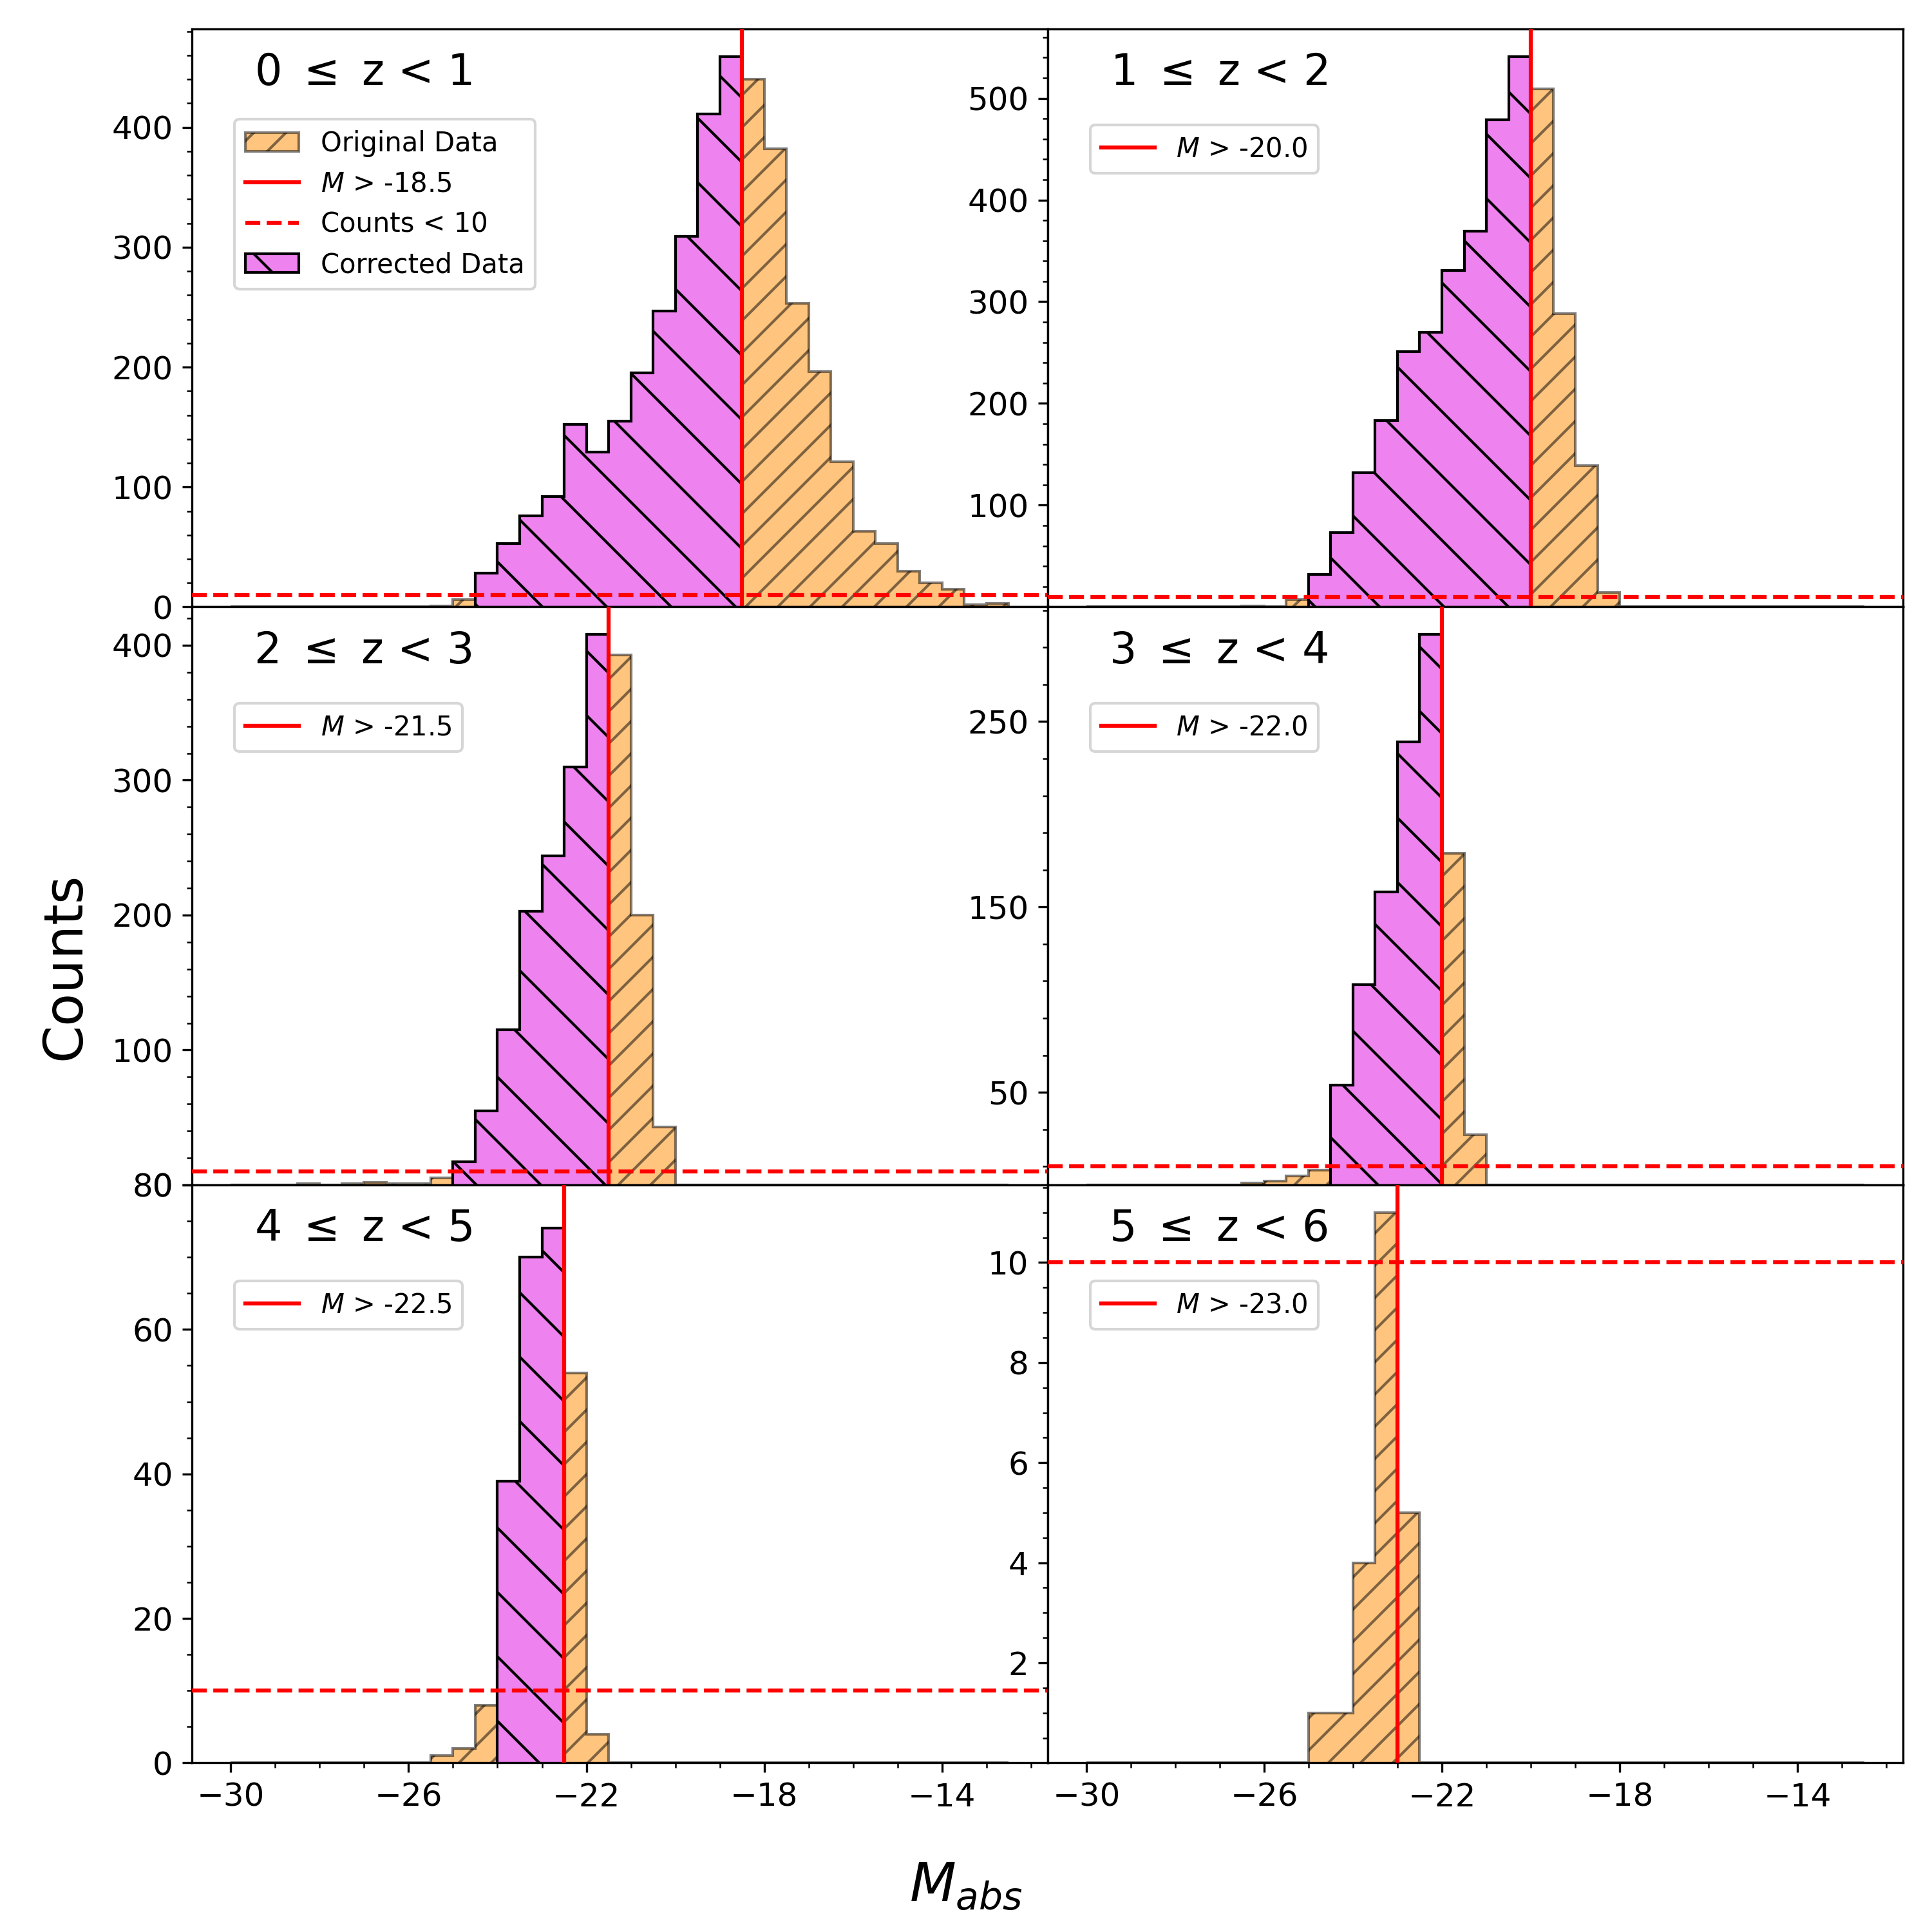
\includegraphics[width=\textwidth]{Figures/Magnitude Counts.png}
    \caption{Number counts in each redshift and luminosity bin. The red vertical line represents the completeness limit. The red dashed horizontal line shows that each luminosity bin requires at least 10 galaxies or is discarded. Purple bins show the corrected data.}
    \label{Fig: Magnitude Counts}
\end{figure}

The maximum comoving distance of each galaxy is then calculated. \Cref{Fig: Magnitude Distribution} (bottom) displays the maximum $d_C$ distance. Galaxies above the $d_L$ maximum line are outside the completeness limit and are removed. Only the first redshift bin, $0 \leq z < 1$, has galaxies faint enough such that their maximum distance does not reach the end of the redshift bin. 

% After removing sources outside the completeness limit, the maximum comoving distance of each galaxy is the end of the redshift bin in which it resides. 

\begin{figure}[t!]
    \centering
    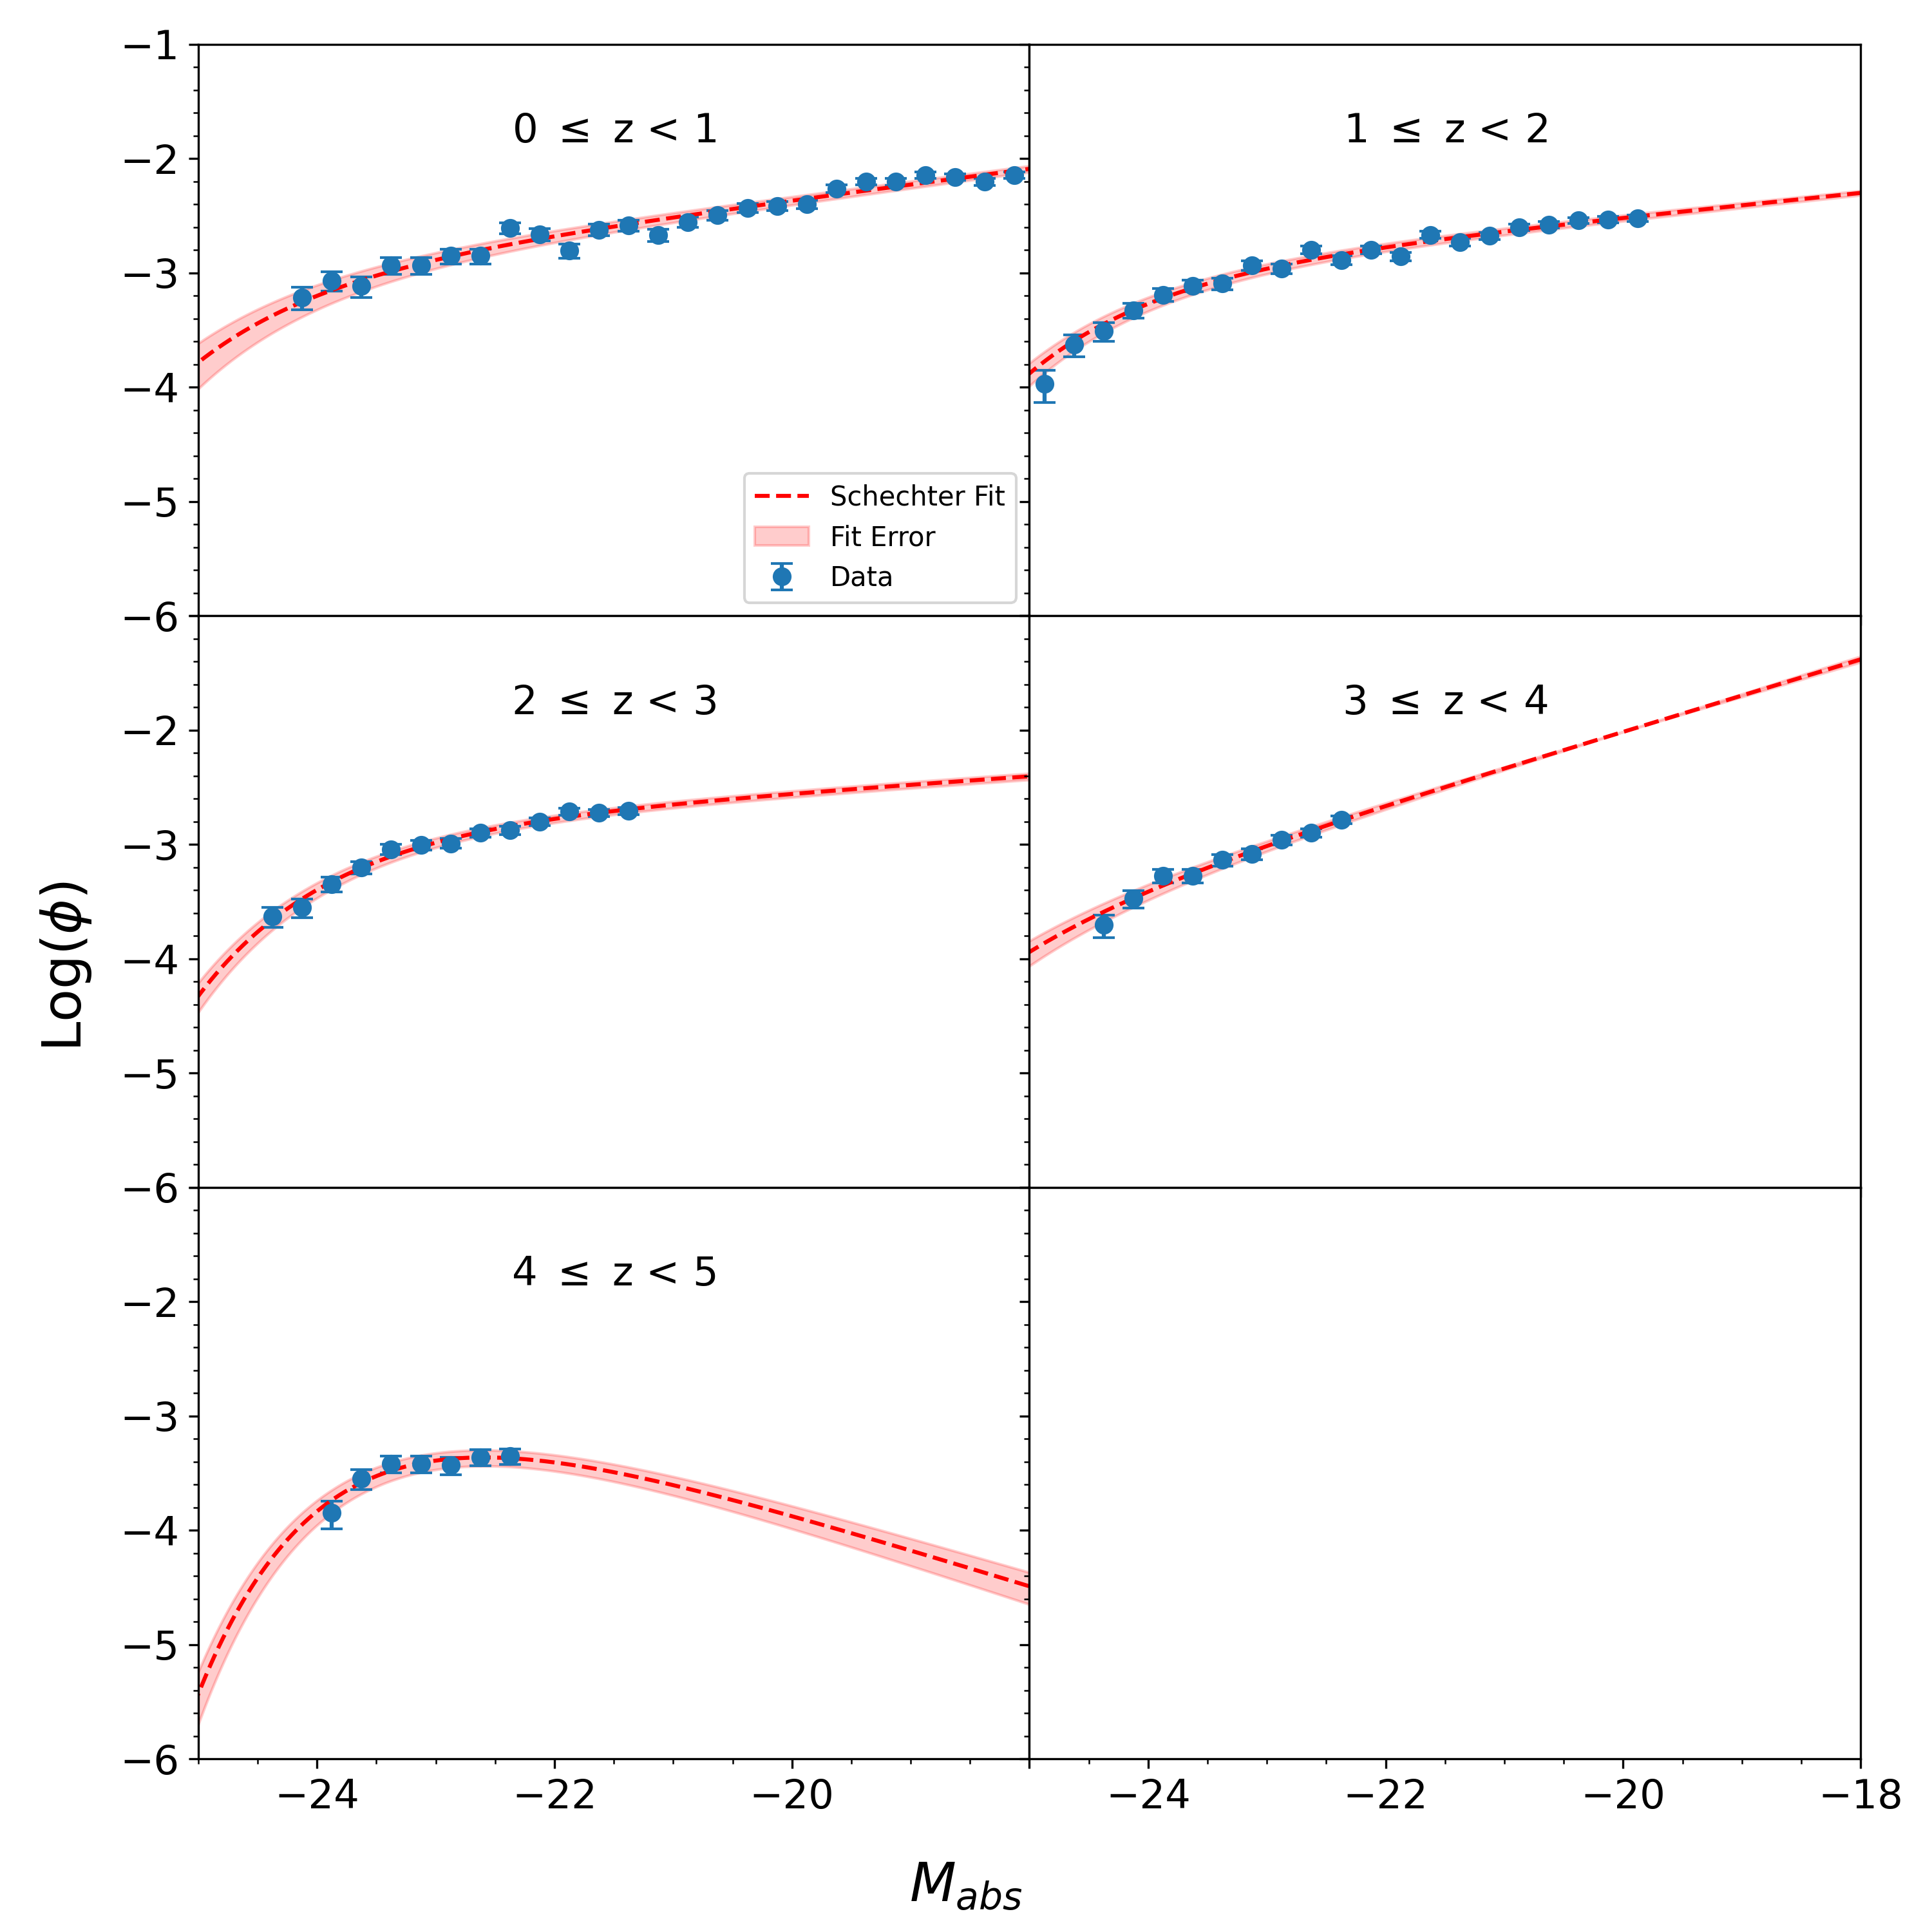
\includegraphics[width=\linewidth]{Figures/Magnitude Function.png}
    \caption{The Magnitude Function of the ZFOURGE \texttt{Ks} band, Evolution across five redshift bins is visualised. The magnitude variant of the Schechter function is fit to the luminosity bins in each redshift bin as the red dashed line. Blue data points are the numbder density values calculated with equation \ref{EQ: Number Density} and $1\sigma$ errors calculated with equation \ref{EQ: Number Density Error}. The red colour-fill represents the uncertainty of the fit based on the error of each luminosity bin. The luminosity bin errors are simply the $1\sigma$ Poisson errors and do not account for flux errors in \texttt{Ks} or photometric redshift errors.}
    \label{fig: Magnitude Function}
\end{figure}

Using number density turnover as the luminosity completeness limit works well because it accounts for Malmquist bias at fainter luminosities. Otherwise, there is a turnover in the number counts as seen in \cref{Fig: Magnitude Counts}. This corrected number count figure represents the shape the \gls{lf} will take. The red vertical line represents the completeness limit. Bins are also discarded if the number of galaxies is less than 10, represented by the red dashed horizontal line. Bins coloured orange fall below the luminosity completeness and count limit. Purple bins are complete and will be used to calculate the \gls{lf}. The final redshift bin, $5 \leq z < 6$, is entirely masked as no bin has more than 10 sources. Several redshift bin sizes are chosen in the literature, such as equal spacing in \textit{look-back time} \citep{thorne_deep_2022}. However, it was decided to use equally spaced redshift bins to simplify the testing process. 

\Cref{fig: Magnitude Function} presents the Magnitude Function of the Ks band in the ZFOURGE \citep{straatman_fourstar_2016} survey in the CDFS field. A specialised Schechter function in absolute magnitude space is fit to each redshift bin, given by the following \Cref{EQ: Magnitude Schechter}:

\begin{equation}
    \phi_{M} = \phi^{*}\times 10^{(-0.4(1-\alpha)(M-M^{*}))} \times \exp{(-10^{-0.4(M-M^{*})})}
    \label{EQ: Magnitude Schechter}
\end{equation}
\myequations{Schechter Magnitude Function}

This equation is found by substituting \Cref{EQ: Absolute Magnitude} into \Cref{EQ: Shechter Function}. The Schechter function of \cref{fig: Magnitude Function} is colour-filled between the luminosity bins' upper and lower uncertainty errors. These errors represent the simple $1\sigma$ Poisson errors, which do not account for errors in the flux of the Ks band or photometric redshift error, which are likely to increase the error. We omit these errors in this section because it is not the primary goal of these tests. Instead, we implement extra sources of error for the decomposed \gls{lf} in \Cref{Sec: Paper Chapter}. The evolution of each redshift bin is evident. Fainter luminosity bins have higher number densities than brighter counterparts, and all decline in number density as redshift increases. Above redshift $z>4$, the Schechter function predicts the number count of faint galaxies to decline rapidly. However, it is not clear that this trend is accurate, as faint sources are entirely lacking at the faint end of the magnitude function. From knowledge of \gls{lss} theory \citep{coil_large-scale_2013}, there should be an abundance of dwarf galaxies at higher redshifts. It is, therefore, highly likely that our final redshift bin $4\leq z < 5$ suffers from incompleteness.